\begin{figure*}
	\centering
	\begin{adjustbox}{width=\textwidth}
		\begin{tikzpicture}[auto]
			\tikzstyle{diff} = [draw, circle, scale=0.5]
			\foreach \Sigma in {0,...,5} {
					\node[yshift=-350+\Sigma*30, yslant=0.5, xslant=-1.5, scale=1] (bertrand-blur-\Sigma-1) {
						\includegraphics[width=.15\textwidth]{figures/registration/sift/bertrand_sigma_\Sigma.png}
					};
				}
			\foreach \Sigma in {0,...,5} {
					\node[yshift=-160+\Sigma*20, xshift=30, yslant=0.5, xslant=-1.5, scale=0.5] (bertrand-blur-\Sigma-2) {
						\includegraphics[width=.15\textwidth]{figures/registration/sift/bertrand_sigma_\Sigma.png}
					};
				}
			\foreach \Sigma in {0,...,5} {
					\node[yshift=-50+\Sigma*20, yslant=0.5, xshift=30, xslant=-1.5, scale=0.25] (bertrand-blur-\Sigma-3) {
						\includegraphics[width=.15\textwidth]{figures/registration/sift/bertrand_sigma_\Sigma.png}
					};
				}

			\foreach \Sigma in {1,...,5} {
			\begin{scope}[
					yshift=-365+\Sigma*30, xshift=280,every node/.append style={
							yslant=0.5, xslant=-1.5},yslant=0.5, xslant=-1.5
				]
				\node[] (bertrand-dog-\Sigma-1) {
					\includegraphics[width=.15\textwidth]{figures/registration/sift/dog_bertrand_sigma_\Sigma.png}
				};
				\ifnum \Sigma>2
					\foreach \x in {-.8,-.6,-.4}  {
							\foreach \y in {-.8,-.6,-.4} {
									\fill[red!50] (\x,\y) rectangle (\x+.2,\y+.2);
								}
						}
				\fi;

			\end{scope}
			\ifnum \Sigma>2 {
				\draw[yshift=-365+\Sigma*30, step=2mm, xshift=280, black, yslant=0.5, xslant=-1.5] (-1,-1) grid (0,0);
				\draw[yshift=-365+\Sigma*30, xshift=280, black, yslant=0.5, xslant=-1.5] (-1,-1) rectangle (0,0);

				}
			\fi;
			\ifnum \Sigma=4
				\fill[green, yshift=-365+\Sigma*30, xshift=280, yslant=0.5, xslant=-1.5] (-.6,-.6) rectangle (-.4,-.4)
			\fi;
			}
			\foreach \Sigma in {1,...,5} {
					\node[yshift=-365+\Sigma*30, xshift=140, diff] (diff-\Sigma-1){\Large$-$};
				}



			\foreach \Sigma in {1,...,5} {
					\node[yshift=-170+\Sigma*20, xshift=250, yslant=0.5, xslant=-1.5, scale=0.5] (bertrand-dog-\Sigma-2) {
						\includegraphics[width=.15\textwidth]{figures/registration/sift/dog_bertrand_sigma_\Sigma.png}
					};
				}
			\foreach \Sigma in {1,...,5} {
					\node[yshift=-170+\Sigma*20, xshift=140, diff] (diff-\Sigma-2){\Large$-$};
				}



			\foreach \Sigma in {1,...,5} {
					\node[yshift=-45+\Sigma*20, xshift=250, yslant=0.5, xslant=-1.5, scale=0.25] (bertrand-dog-\Sigma-3) {
						\includegraphics[width=.15\textwidth]{figures/registration/sift/dog_bertrand_sigma_\Sigma.png}
					};
				}
			\foreach \Sigma in {1,...,5} {
					\node[yshift=-45+\Sigma*20, xshift=140, diff] (diff-\Sigma-3){\Large$-$};
				}
			%		($(diff-\Sigma-\x) + (0,5mm)$)
			% draw annotations
			\foreach \x in {1,2,3} {
					\foreach \Sigma in {1,...,5} {
							\draw[-] (bertrand-blur-\Sigma-\x) edge (diff-\Sigma-\x);
						}
					\foreach \Sigma in {0,...,4} {
							\pgfmathtruncatemacro{\nodelabel}{1+\Sigma}
							\draw[-] (bertrand-blur-\Sigma-\x) edge (diff-\nodelabel-\x);
						}
					\foreach \Sigma in {1,...,5} {
							\draw[->] (diff-\Sigma-\x) edge (bertrand-dog-\Sigma-\x);
						}
				}
			\coordinate (a) at (-.5, -.5);
			\node (keypoint) [right] at (10,-6) {Candidate Keypoint (not to scale)};
			\tikzstyle{trans} = [thick,->,>=stealth]
			\path[trans] ([] bertrand-blur-3-2.north west) edge[bend left, out=120, in=90] node[above, sloped] {Down-sample 2x} ([] bertrand-blur-0-3.north west);
			\path[trans] ([xshift=2mm] bertrand-blur-3-1.north west) edge[bend left, out=120, in=90] node[above, sloped] {Down-sample 2x} ([] bertrand-blur-0-2.north west);

			\path[trans] ([] keypoint) edge[] node[] {} ([yshift=-365+4*30, xshift=280, yslant=0.5, xslant=-1.5] a);
			\foreach \x in {0,...,4} {
					\pgfmathtruncatemacro{\nodelabel}{\x+1}
					\path[trans] ([xshift=-10mm] bertrand-blur-\x-1.north west) edge[bend left] node[above, sloped] {$k^{\nodelabel}\sigma$} ([xshift=-10mm] bertrand-blur-\nodelabel-1.north west);
				}
		\end{tikzpicture}
	\end{adjustbox}
	\caption{The imaging model illustrating the relationship between a scene and final low-resolution images due to noise, motion, blur, and sampling.}
	\label{fig:bertrand}
\end{figure*}
Images obtained from multiple vantage points, or at different times, of the same scene, become distorted with respect
to each other.
%
Since in MISR the aim is to exploit new information across multiple LR samples we need to first rectify these distortions and reconcile the images.
%
Effectively this means finding one or more pixel transformations that enable mapping all LR images to a common pixel grid.
%
When the transformations cannot be deduced from first principles (e.g. precise knowledge of the relative motion of the scene and the imaging system) they must be estimated from the LR images.
%
There are broadly two perspectives on constructing the transformation \(f\) (see eqn.~\eqref{eqn:registration}): the global perspective which aims to model motion as a map of the image as a whole and the local perspective which aims to model motion as a deformation of individual pixels.
%
These two perspectives naturally correspond to a globally or locally defined transformation \(f\).
%
We first cover global algorithms, examining the different techniques available for each step, and then move on to local algorithms.

\subsection{Global Algorithms}

Most global image registration algorithms consist of a feature detection and selection step (also called Control Point (CP) selection), a feature matching step, and a transform estimation step.
%

\subsubsection{Feature Detection and Selection}

Feature detection and selection is the process of identifying features of the image that are presumed to be invariant across the multiple images to registered.
%
Note that here by features we mean image artifacts (e.g. edges, contours, line intersections, or corners); in this context encodings or transformations of these image artifacts are called \textit{descriptors}.
%
The CPs are the data that will be used to estimate the transformation \(f\).
%
Therefore, in order that the estimated transformation is accurate, CPs should be robust to noise and image degradation, sufficiently distributed throughout the image, and readily matched in the matching step.

\paragraph{Harris Corner Detection}
Bentoutou \etal\cite{bentoutou2005automatic} use a Harris detector\cite{harris1988combined} to find corner points, arguing that corners are robust to noise and stable over multiple images.
%
The Harris detector improves on the Moravec\cite{moravec1980obstacle} detector.
%
The Moravec detector starts from the error function \(E_{x,y}(u,v)\) which computes the sum of the squared differences (SSD) between an \(m \times m\) weighted window around a pixel \(X(x, y)\) and weighted windows shifted by \(u,v\) pixels:
\begin{multline}
	\quad E_{x,y}(u,v) \coloneqq \\ \sum_{i,j=-m/2}^{m/2} w_{ij}\left[ X(x_i+ u,y_j+v) - X(x_i, y_j)\right]^2
	\label{moravecerrorfunction}
\end{multline}
where \(x_i \coloneqq x + i\) and \(y_j \coloneqq y+j\).
\begin{figure}
	\centering
	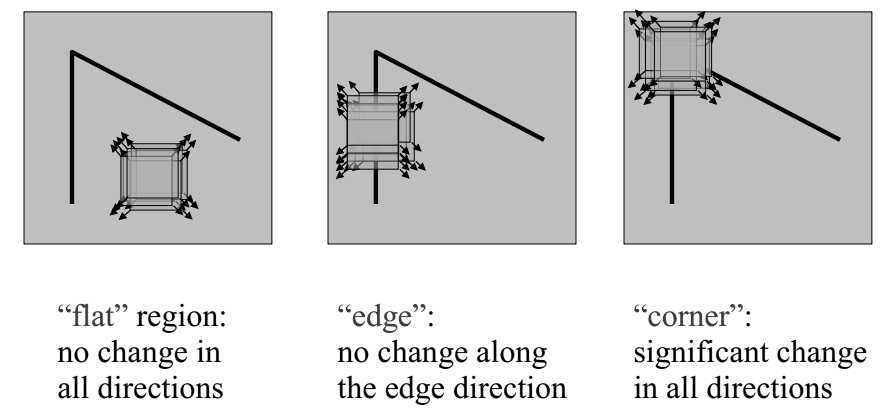
\includegraphics[width=\linewidth,keepaspectratio]{figures/registration/corners.png}
	\caption{Moravec Corner Detector}
	\label{fig:corners}
\end{figure}
Moravec assigns a "corner score" according to the following reasoning (see figure~\ref{fig:corners}):
\begin{enumerate}
	\item If a pixel is in a region of uniform intensity then \(E_{x,y}(u,v)\) is small for all \(u,v\) (since neighboring windows are similar).
	\item If a pixel is on an edge, then \(E_{x,y}(u,v)\) for either \(u > 0\) or \(v > 0\), but not both, is high.
	\item If a pixel is on a corner, then \(E_{x,y}(u,v)\) for \(u > 0\) and \(v > 0\) is high.
\end{enumerate}
Therefore the corner score at pixel coordinate \((x,y)\) is \(\min_{u,v} E_{x,y}(u,v)\) in order to select for the third case.
%
Moravec comments that this corner score is not isotropic, i.e. if edges aren't aligned with either the pixel axes or diagonals then \(E_{x,y}(u,v)\) will incorrectly be low.
%
Harris' insight was to linearize \(E_{x,y}(u,v)\) in order to compute a quantity more closely related to the intensity variation in a local
neighborhood of a pixel:
\begin{equation}
	X(x_i + u,y_j + v) \approx  X(x_i,y_j) + \frac{\partial X}{\partial u}u + \frac{\partial X }{\partial v} v
\end{equation}
where the partial derivatives are taken at \((x,y)\).
%
This implies
\begin{align}
	E_{x,y}(u,v) & \approx \sum_{i,j=-m/2}^{m/2} w_{ij} \left[ X_u u + X_v v\right]^2                 \\
	             & = \sum_{i,j=-m/2}^{m/2} w_{ij} \left[ X_u^2 u^2 + X_v^2 v^2 + 2 X_u X_v u v\right] \\
	             & = \left[ u,v \right] \begin{bmatrix}
		\sum w_{ij}X_u^2   & \sum w_{ij}X_u X_v \\
		\sum w_{ij}X_u X_v & \sum w_{ij}X_v^2   \\
	\end{bmatrix}  \begin{bmatrix}
		u \\
		v
	\end{bmatrix}          \\
	             & = \left[ u,v \right] M  \begin{bmatrix}
		u \\
		v
	\end{bmatrix} \label{eqn:structurematrix}
\end{align}
where \(X_u = \partial X/\partial u\) and similarly \(X_v\).
%
The matrix in eqn.~\eqref{eqn:structurematrix}, called the \textit{structor tensor} or \textit{second-moment matrix} \(M\), is the quantity Harris investigated.
%
Harris reasoned that the cases of Moravec correspond to conditions on the eigenvalues \(\lambda_1, \lambda_2\) of \(M\):
\begin{enumerate}
	\item If \(\lambda_1 \approx \lambda_2 \approx 0\) then \(X(x,y)\) is in a region of uniform intensity.
	\item If \(\lambda_1 \gg \lambda_2\) or \(\lambda_2 \gg \lambda_1\) then \(X(x,y)\) is on an edge.
	\item \(\lambda_1 \approx \lambda_2 > 0\) then \(X(x,y)\) is on a corner.
\end{enumerate}
Notice that if \(w_{ij} = 1\) then this is just the gradient covariance of the image and the Harris detector is essentially a local Principle Components Analysis (PCA).
%
In fact Harris doesn't actually compute the eigenvalues but instead a related quantity called the "strength":
\begin{align}
	S & = \lambda_1 \lambda_2 - \kappa (\lambda_1 + \lambda_2)^2 \\
	  & = \det(M) - \kappa \operatorname{trace}^2(M)
	\label{eqn:strength}
\end{align}
%
Hence Bentoutou \etal~first compute a gradient map of the image using a first order Gaussian derivative filter.
%
They then threshold\anote{threshold} the gradient map at the average gradient value, thereby extracting only sufficiently "interesting" regions, and compute the strength \(S\) for all pixels.
%
They also apply Non-maximum Suppression\anote{nms} (NMS) using a \(3 \times 3\) window and further threshold the remaining non-zero strength values at a threshold of 1\% of maximum observed strength.
%
Finally only the "strongest" \(n\) corners are kept.

\paragraph{SIFT}

\begin{figure}
	\centering
	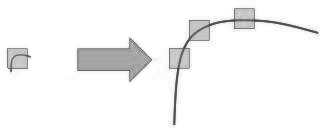
\includegraphics[width=\linewidth,keepaspectratio]{figures/registration/sift/sift_scale_invariant.png}
	\caption{Harris Detector failing to recognize the right image as a corner.}
	\label{fig:sift_harris}
\end{figure}
One issue with Harris detectors is that they're not invariant to scale (see figure~\ref{fig:sift_harris}).
%
Zahra \etal\cite{zahrasift} resolves this issue by using the Scale Invariant Feature Transform\cite{lowe2004distinctive} (SIFT) to identify CPs that, as the name implies, are invariant across multiple scales.
%
SIFT identifies scale invariant and noise robust features of an image, called \textit{keypoints}, by first finding candidate points with high local curvature at multiple scales and then culling according to some heuristics.
\begin{figure*}
	\pgfplotstableread[]{figures/registration/sift/subgrad_hists.csv}\subgradhists;
	\tikzstyle{every picture}+=[remember picture]
	\tikzset{
		pics/greensquare/.style args={#1/#2/#3}{
				code = {
						\draw[green, line width=.5mm] (#1,#2) rectangle (#1+#3, #2+#3);
					}
			},
		subgradbin/.pic={
				\foreach \i in {0.0, 1.0} {
						\pgfmathsetmacro{\x}{0.5+\i*2*.08825};
						\foreach \j in {0.0, 1.0} {
								\pgfmathsetmacro{\y}{0.5+\j*2*.08825};
								\pic[] {greensquare=\x/\y/2*.08825};
							};
					};
			},
		pics/subgradbins/.style args={#1}{
				code = {
						\foreach \x in {0,1,2,3} {
								\pgfmathtruncatemacro{\angle}{#1+\x*90}
								\pic[rotate around={\angle:(0.5,0.5)}] {subgradbin};
							}
					}
			},
		pics/edgehistogram/.style args={#1/#2}{
				code={
						\begin{axis}[area style, width=2.5cm,height=2.5cm, hide axis, at={(#1cm,#2cm)}]
							\addplot+[ybar interval] plot coordinates {
									(-0.50, 2) (0.5, 4) (1.5, 5) (2.5, 3) (3.5, 2) (4.5, 2) (5.5, 0)
								};
							\path
							\foreach[count=\i from 0] \v in {2, 4, 5, 3, 2, 2} {
									(\i, \v) node[below] {\tiny\v}
								};
						\end{axis}
					}
			},
		pics/randomedgehistogram/.style args={#1/#2}{
				code={
						\node (hist-#1#2) at (#1cm+.5cm,#2cm+.5cm) {};% {#1,#2};
						\begin{axis}[area style, width=2.5cm,height=2.5cm, hide axis, at={(#1cm,#2cm)}]
							\pgfmathtruncatemacro{\rowindex}{#1*4+#2}
							\pgfplotstablegetelem{\rowindex}{[index]0}\of{\subgradhists}\pgfmathtruncatemacro{\na}{\pgfplotsretval};
							\pgfplotstablegetelem{\rowindex}{[index]1}\of{\subgradhists}\pgfmathtruncatemacro{\nb}{\pgfplotsretval};
							\pgfplotstablegetelem{\rowindex}{[index]2}\of{\subgradhists}\pgfmathtruncatemacro{\nc}{\pgfplotsretval};
							\pgfplotstablegetelem{\rowindex}{[index]3}\of{\subgradhists}\pgfmathtruncatemacro{\nd}{\pgfplotsretval};
							\pgfplotstablegetelem{\rowindex}{[index]4}\of{\subgradhists}\pgfmathtruncatemacro{\ne}{\pgfplotsretval};
							\pgfplotstablegetelem{\rowindex}{[index]5}\of{\subgradhists}\pgfmathtruncatemacro{\nf}{\pgfplotsretval};
							\pgfplotstablegetelem{\rowindex}{[index]6}\of{\subgradhists}\pgfmathtruncatemacro{\ng}{\pgfplotsretval};
							\pgfplotstablegetelem{\rowindex}{[index]7}\of{\subgradhists}\pgfmathtruncatemacro{\nh}{\pgfplotsretval};
							\addplot+[ybar interval] plot coordinates {
									(-0.50, \na)
									(0.5, \nb)
									(1.5, \nc)
									(2.5, \nd)
									(3.5, \ne)
									(4.5, \nf)
									(5.5, \ng)
									(6.5, \nh)
									(7.5, 0)
								};
							\draw
							\foreach[count=\i from 0] \v in {\na, \nb, \nc, \nd, \ne, \nf, \ng, \nh} {
									(\i, \v) node[below] {\scalebox{.3}{\v}}
								};
						\end{axis}
					}
			},
		array/.style={
				draw,
				minimum width=2em,
				minimum height=2em,
				outer sep=0pt
			},
	}
	\newcommand*{\siftwidth}{.5\linewidth}
	\newcommand*{\length}{sqrt((2.*x^2+2.*y^2)^2 + (8.*x^2*y^2)^2 )}
	\pgfplotsset{
		dominantorientationaxis/.style={
				enlargelimits = false,
				view={0}{90},
				xmin=0, xmax=1, ymin=0, ymax=1,
				ytick distance=1/16,
				xtick distance=1/16,
				axis equal image, grid=both,
				minor grid style={black},
				major grid style={black},
				axis equal image,
			},
	}
	\pgfplotsset{ticks=none}
	\begin{subfigure}{\siftwidth}
		\centering
		\begin{tikzpicture}
			\begin{axis}[dominantorientationaxis]
				\addplot[on layer=axis background] graphics[xmin=0, xmax=1, ymin=0, ymax=1]
					{figures/registration/sift/bert_keypoint.png};
				\addplot[redarrow,quiver={u=\thisrow{u},v=\thisrow{v}}] table {figures/registration/sift/grads.csv};
				\node[dot=5pt](keypoint) at (0.5,0.5) {};
			\end{axis}
			\node (keyp) at (4,6.5) {Keypoint};
			\draw[redarrow] (keyp)--(keypoint);
		\end{tikzpicture}
		\caption{Keypoint neighborhood.} \label{fig:siftdescriptora}
	\end{subfigure}
	\pgfmathsetmacro{\rot}{54}
	\pgfmathsetmacro{\br}{sqrt(2)*.5/2}
	\begin{subfigure}{\siftwidth}
		\centering
		\begin{tikzpicture}
			\begin{axis}[dominantorientationaxis, set layers]
				\addplot[on layer=axis background] graphics[xmin=0, xmax=1, ymin=0, ymax=1]
					{figures/registration/sift/bert_keypoint.png};
				\addplot[redarrow,quiver={u=\thisrow{u},v=\thisrow{v}}] table {figures/registration/sift/grads.csv};
				\node[dot=5pt](keypoint) at (0.5,0.5) {};

				\draw[yellow] (0.5, 0.5) circle [radius=.5];
				\pic[rotate around={\rot:(0.5,0.5)}] {greensquare=.1464/.1464/.707};
				\draw[line width=2pt,red,-latex](.5,.5)--(.5+0.3579, 1);
				\coordinate (gausscircle) at (.75,.25);
				\coordinate (dominantgrad) at (.5+0.25,.5+.35);
				\coordinate (gradsquare) at (.5-\br,.5+\br);
			\end{axis}
			\node (gausswin) at (5,-0.5) {Gradient Window};
			\node (gradwin) at (1,6.5) {Gaussian Window};
			\node (domin) at (4,6.5) {Majority Gradient};
			\draw[redarrow] (gausswin)--(gausscircle);
			\draw[redarrow] (gradwin)--(gradsquare);
			\draw[redarrow] (domin)--(dominantgrad);
		\end{tikzpicture}
		\caption{Oriented and filterd keypoint gradient neigbhorhood.} \label{fig:siftdescriptorb}
	\end{subfigure}
	\vskip\baselineskip
	\begin{subfigure}{\siftwidth}
		\centering
		\begin{tikzpicture}
			\begin{scope}[rotate=\rot,transform shape,local bounding box=scope1]
				\clip[](1.95,1.99) rectangle (6.0,6.03);
				\begin{axis}[dominantorientationaxis, rotate around={-\rot:(.5,.5)}, grid=none]
					\addplot[on layer=axis background] graphics[xmin=0, xmax=1, ymin=0, ymax=1]
						{figures/registration/sift/bert_keypoint.png};
					\addplot[redarrow,quiver={u=\thisrow{u},v=\thisrow{v}}] table {figures/registration/sift/grads.csv};
					\pic[] {subgradbins=\rot};
					\node[dot=5pt](keypoint) at (0.5,0.5) {};
				\end{axis}
			\end{scope}
			\begin{scope}[shift={($(scope1.south)-(0,1cm)$)}]
				\coordinate (gradbin) at (0.5,5.5);
				\node (gradb) at (2,6.5) {Gradient bin};
				\draw[redarrow] (gradb)--(gradbin);
			\end{scope}
		\end{tikzpicture}
		\caption{16 Keypoint neigbhorhood gradient bins.} \label{fig:siftdescriptorc}
	\end{subfigure}
	\begin{subfigure}{\siftwidth}
		\centering
		\begin{tikzpicture}
			\begin{scope}[rotate=\rot,transform shape,local bounding box=scope1]
				\foreach \i [evaluate=\i as \x using \i*1.0] in {0,...,3}{
						\foreach \j [evaluate=\j as \x using \j*1.0] in {0,...,3}{
								\pic {greensquare=\i/\j/1.0};
								\pic {randomedgehistogram=\i/\j};
							}
					}
				\node[dot=5pt](keypoint) at (2.0,2.0) {};
			\end{scope}
			\node (histb) at (2,5.5) {Histogram of gradient orientations};
			\draw[redarrow] (histb)--(hist-32);
			\begin{scope}[shift={($(scope1.south)-(0,1cm)$)}]
				\matrix (A) [matrix of math nodes, nodes={array, anchor=center}, column sep=-\pgflinewidth] {
					\pgfmathtruncatemacro{\rowindex}{3}
					\pgfplotstablegetelem{\rowindex}{[index]0}\of{\subgradhists}\pgfmathprintnumber[fixed,precision=0]{\pgfplotsretval},
					\pgfplotstablegetelem{\rowindex}{[index]1}\of{\subgradhists}\pgfmathprintnumber[fixed,precision=0]{\pgfplotsretval},
					\pgfplotstablegetelem{\rowindex}{[index]2}\of{\subgradhists}\pgfmathprintnumber[fixed,precision=0]{\pgfplotsretval},
					\pgfplotstablegetelem{\rowindex}{[index]3}\of{\subgradhists}\pgfmathprintnumber[fixed,precision=0]{\pgfplotsretval},
					\pgfplotstablegetelem{\rowindex}{[index]4}\of{\subgradhists}\pgfmathprintnumber[fixed,precision=0]{\pgfplotsretval},
					\pgfplotstablegetelem{\rowindex}{[index]5}\of{\subgradhists}\pgfmathprintnumber[fixed,precision=0]{\pgfplotsretval},
					\pgfplotstablegetelem{\rowindex}{[index]6}\of{\subgradhists}\pgfmathprintnumber[fixed,precision=0]{\pgfplotsretval},
					\pgfplotstablegetelem{\rowindex}{[index]7}\of{\subgradhists}\pgfmathprintnumber[fixed,precision=0]{\pgfplotsretval} &
					\pgfmathtruncatemacro{\rowindex}{2}
					\pgfplotstablegetelem{\rowindex}{[index]0}\of{\subgradhists}\pgfmathprintnumber[fixed,precision=0]{\pgfplotsretval},
					\pgfplotstablegetelem{\rowindex}{[index]1}\of{\subgradhists}\pgfmathprintnumber[fixed,precision=0]{\pgfplotsretval},
					\pgfplotstablegetelem{\rowindex}{[index]2}\of{\subgradhists}\pgfmathprintnumber[fixed,precision=0]{\pgfplotsretval},
					\pgfplotstablegetelem{\rowindex}{[index]3}\of{\subgradhists}\pgfmathprintnumber[fixed,precision=0]{\pgfplotsretval},
					\pgfplotstablegetelem{\rowindex}{[index]4}\of{\subgradhists}\pgfmathprintnumber[fixed,precision=0]{\pgfplotsretval},
					\pgfplotstablegetelem{\rowindex}{[index]5}\of{\subgradhists}\pgfmathprintnumber[fixed,precision=0]{\pgfplotsretval},
					\pgfplotstablegetelem{\rowindex}{[index]6}\of{\subgradhists}\pgfmathprintnumber[fixed,precision=0]{\pgfplotsretval},
					\pgfplotstablegetelem{\rowindex}{[index]7}\of{\subgradhists}\pgfmathprintnumber[fixed,precision=0]{\pgfplotsretval} &
					\cdots\cdots\cdots                                                  &
					\pgfmathtruncatemacro{\rowindex}{12}
					\pgfplotstablegetelem{\rowindex}{[index]0}\of{\subgradhists}\pgfmathprintnumber[fixed,precision=0]{\pgfplotsretval},
					\pgfplotstablegetelem{\rowindex}{[index]1}\of{\subgradhists}\pgfmathprintnumber[fixed,precision=0]{\pgfplotsretval},
					\pgfplotstablegetelem{\rowindex}{[index]2}\of{\subgradhists}\pgfmathprintnumber[fixed,precision=0]{\pgfplotsretval},
					\pgfplotstablegetelem{\rowindex}{[index]3}\of{\subgradhists}\pgfmathprintnumber[fixed,precision=0]{\pgfplotsretval},
					\pgfplotstablegetelem{\rowindex}{[index]4}\of{\subgradhists}\pgfmathprintnumber[fixed,precision=0]{\pgfplotsretval},
					\pgfplotstablegetelem{\rowindex}{[index]5}\of{\subgradhists}\pgfmathprintnumber[fixed,precision=0]{\pgfplotsretval},
					\pgfplotstablegetelem{\rowindex}{[index]6}\of{\subgradhists}\pgfmathprintnumber[fixed,precision=0]{\pgfplotsretval},
					\pgfplotstablegetelem{\rowindex}{[index]7}\of{\subgradhists}\pgfmathprintnumber[fixed,precision=0]{\pgfplotsretval}
					\\};
				\draw[decorate,decoration={brace, amplitude=10pt, raise=5pt, mirror}]
				(A-1-1.south west) to node[black,midway,below= 15pt] {$16 \times 8 = 128$ entries} (A-1-4.south east);%
				\draw[redarrow] (hist-03) -- (A-1-1);
				\draw[redarrow] (hist-02) -- (A-1-2);
				\draw[redarrow] (hist-01) -- (A-1-3);
				\draw[redarrow] (hist-00) -- (A-1-3);
				\foreach \i in {1,...,2}{
						\foreach \j in {0,...,3}{
								\draw[redarrow] (hist-\i\j) -- (A-1-3);
							}
					}
				\draw[redarrow] (hist-33) -- (A-1-3);
				\draw[redarrow] (hist-31) -- (A-1-3);
				\draw[redarrow] (hist-32) -- (A-1-3);
				\draw[redarrow] (hist-30) -- (A-1-4);
			\end{scope}
		\end{tikzpicture}
		\caption{Histogram of gradient orientations descriptor.} \label{fig:siftdescriptord}
	\end{subfigure}
	\caption{Sift keypoint descriptor construction.} \label{fig:siftdescriptor}
\end{figure*}


%
It then "describes" these keypoints by a rotation invariant and noise robust representation.
%
The algorithm consists of five steps:
\begin{enumerate}
	\item Scale-space pyramid construction: a sequence of increasingly sub-sampled and more strongly Gaussian filtered images is computed. The sequence of differences of these images is also computed; the sequence of differenced images approximates the multi-scale Laplacian of Gaussians\anote{log} (LoG) of the image (see figure~\ref{fig:siftpyramid}).
	\item Keypoint detection: candidate keypoints are points on edges with curvature, i.e. extrema along scale and space dimensions in the LoG pyramid (see figure~\ref{fig:siftpyramid}).
	\item Keypoint selection: candidate keypoints are more precisely localized using an iterative process. Keypoints of low-contrast (therefore sensitive to noise) or on edges of low curvature\anote{smallcurvature} are culled.
	\item Keypoint orientation assignment: orientation is assigned to each keypoint by taking a weighted majority vote of all gradient orientations in a neighborhood of the keypoint (see figure~\ref{fig:siftdescriptorb}). Large minority votes (80\% of majority) are used to create more keypoints at the same pixel point.
	\item Keypoint descriptor computation: for each keypoint the descriptor is computed by partitioning the keypoint's neighborhood into \(2^k\) sub-neighborhoods, computing an 8-bin histogram of oriented gradients\anote{hog} (HOG) in each sub-neighborhood, and concatenating (see figure~\ref{fig:siftdescriptord}). In Lowe \etal\cite{lowe2004distinctive} \(2^4=16\) sub-neighborhoods are used to produce an \(8\times16 = 128\) entry length descriptor. The descriptor is also normalized to unit length in order to make it invariant to luminance (intensity).
\end{enumerate}
SIFT is indeed effective as a CP detector but unfortunately it is patented.
%
Alternatives include Binary Robust Invariant Scalable Keypoints\cite{leutenegger2011brisk}, and Oriented FAST and rotated BRIEF\cite{rublee2011orb} (which itself consists of applying Features from accelerated segment test\cite{rosten2006machine} to detect points of interest and Binary Robust Independent Elementary Features\cite{calonder2010brief} to compute descriptors).

\subsubsection{Feature Matching}

After robust features are identified in the reference image and the displaced images, they need to be matched.
%
For example for SIFT, where the descriptors are designed to be invariant across images, Euclidean distance using a \(k\)-d tree\anote{kdtree} can be used to efficiently match keypoint descriptors.
%
Although this often leads to false-positive matches (Zahra \etal~resolve this by using Random Sample Consensus (RANSAC)\anote{ransac}) it's a natural feature matching method.
%
In other cases the matching mechanism is not so straightforward; for a class of algorithms called area-based or intensity-based algorithms, that in fact combine the feature detection and matching step into one, matching involves comparing summaries of patches in the reference image and the displaced image.

\paragraph{Normalized Cross-correlation}
The simplest strategy for matching by region is to grid-search\anote{gridsearch} the space of possible translational shifts \(\Delta x, \Delta y\) and assess the quality of the registration for a given shift using a similarity metric.
%
One such similarity metric is Normalized Cross-correlation (NCC); for two image patches \(X, Y\) (with the same width, height) NCC is defined in a straightforward way
\begin{multline}
	NCC(X, Y) = \\ \frac{\sum_{x,y} \left(X(x,y) - \hat{X}\right) \left(Y(x,y) - \hat{Y}\right)}{\sqrt{\sum_{x,y} \left(X(x,y) - \hat{X}\right)^2} \sqrt{ \sum_{x,y} \left(Y(x,y) - \hat{Y}\right)^2 }}
\end{multline}
where \(\hat{X}, \hat{Y}\) are mean patch values.

\begin{figure}[!htbp]
	\begin{subfigure}{\linewidth}
		\centering
		\begin{adjustbox}{width=.8\textwidth}
			\begin{tikzpicture}
				\node[inner sep=0pt, xshift=50, yshift=-50] (shiftedcat) {
					{\transparent{.5}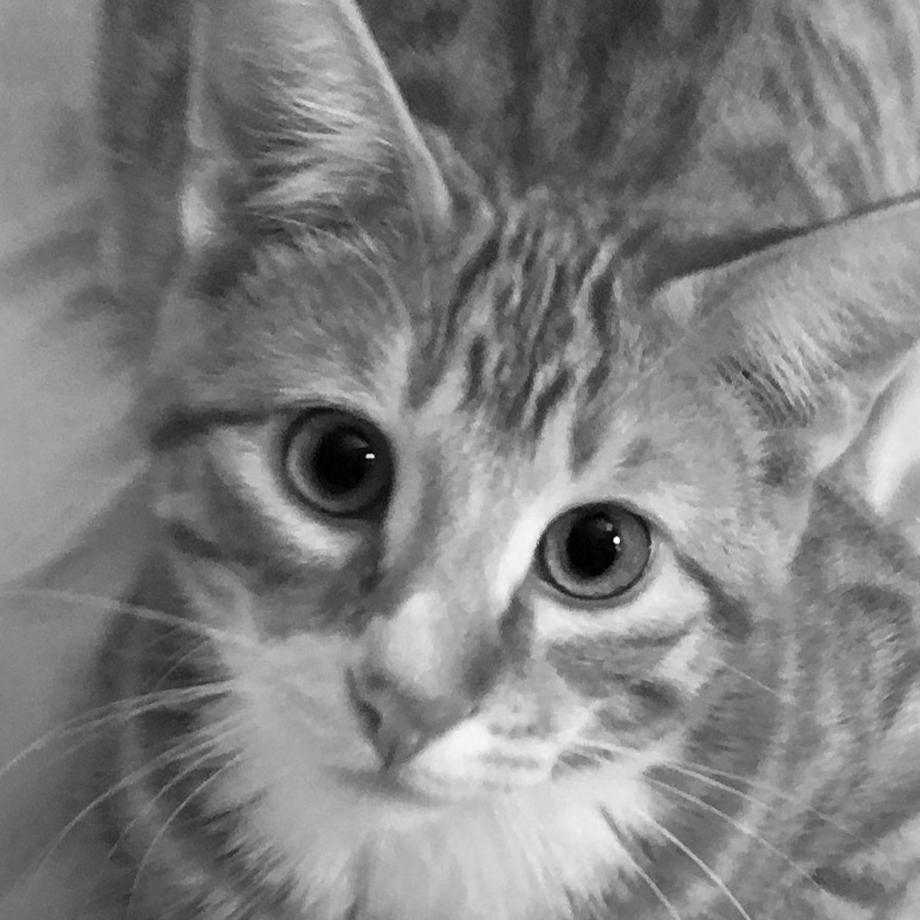
\includegraphics[]
							{figures/registration/cross-correlation/trimmed_cat.jpg}
						}};
				\node[inner sep=0pt, xshift=-50pt, yshift=50pt] (shiftedcat) {
					{\transparent{0.5}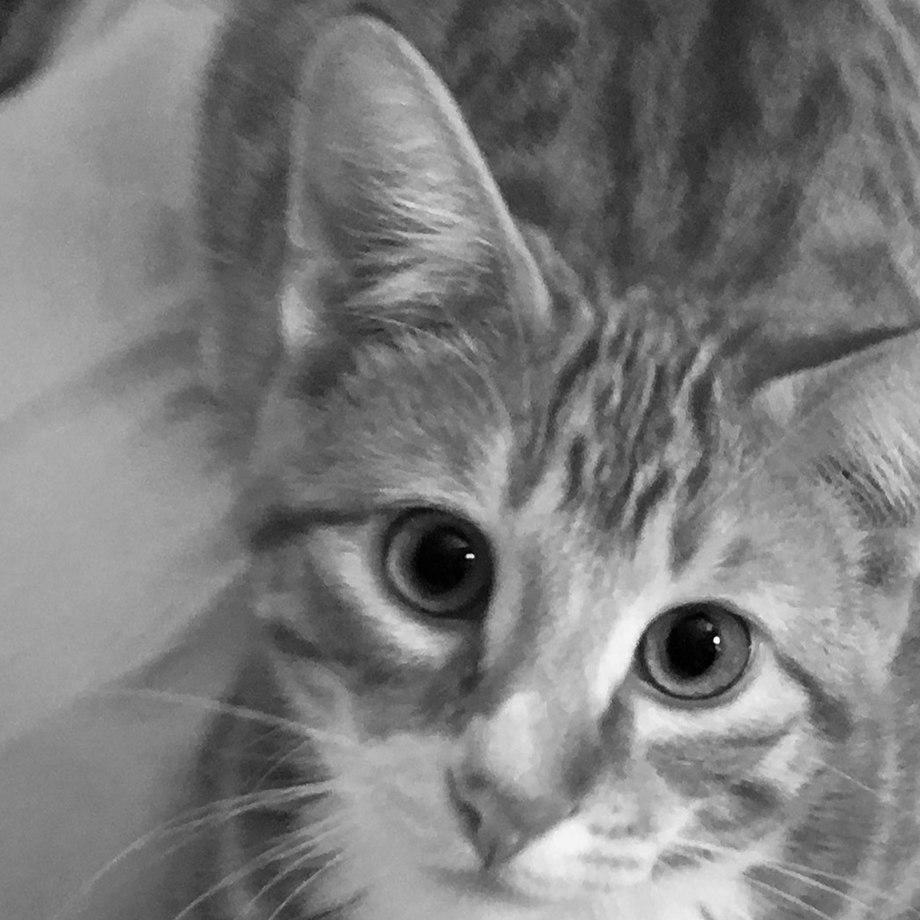
\includegraphics[]
							{figures/registration/cross-correlation/shifted_trimmed_cat.jpg}
						}};
				\draw[red, line width=1mm] (-250pt,-250pt) rectangle (250pt,250pt);
				\node(corrwin) at (0,250pt) {};
				\node[label={[label distance=1cm]:\scalebox{5}{Fixed cross-correlation window}}] (corrw) at (0,600pt) {};
				\draw[redarrow, line width=1mm] (corrw)--(corrwin);
			\end{tikzpicture}
		\end{adjustbox}
		\caption{100 pixel shifted images.} \label{fig:shiftedcat}
	\end{subfigure}
	\vskip\baselineskip
	\begin{subfigure}{\linewidth}
		\centering
		\begin{tikzpicture}
			\begin{axis}
				\addplot3 [surf, mesh/rows=19, mesh/ordering=x varies]
				table[col sep=comma] {figures/registration/cross-correlation/surf.csv};
				\node[above] at (axis cs:-110,-110,224141) {\((-100, -100)\)};
			\end{axis}
		\end{tikzpicture}
		\caption{Cross-correlation for various \(\Delta x, \Delta y\) shifts, with highest correlation at the shift.}
		\label{fig:crosscorr}
	\end{subfigure}
	\vskip\baselineskip
	\begin{subfigure}{\linewidth}
		\centering
		\begin{tikzpicture}
			\begin{axis}
				\addplot3 [surf, mesh/rows=19, mesh/ordering=x varies]
				table[col sep=comma] {figures/registration/cross-correlation/delta_surf.csv};
				\node[above] at (axis cs:-110,-110,1) {\((-100, -100)\)};
			\end{axis}
		\end{tikzpicture}
		\caption{Phase-correlation for various \(\Delta x, \Delta y\) shifts, with single peak at the correct shift.}
		\label{fig:phasecorr}
	\end{subfigure}
	\caption{Cross-correlation feature matching.}
	\label{fig:nccshift}
\end{figure}

%
The NCC image registration technique performs a grid-search over possible shifts and compute the cross-correlation of the shifted images (see figure~\ref{fig:shiftedcat}) (usually over a fixed cross-correlation window rather than the entire image for the sake of computational efficiency).
%
The maximum response as a function \(\Delta x, \Delta y\) is the imputed translation between the images (see figure~\ref{fig:crosscorr}).
%
An alternative but closely related method is \textit{phase correlation}, based on the Fourier shift theorem\anote{fouriershift}  (the value of going to Fourier space is availability of highly optimized algorithms for computing the Fourier transform).
%
Let \(\mathcal{X}(u,v) = \mathcal{F}\{X(x,y)\}, \; \mathcal{Y}(u,v) = \mathcal{F}\{Y(x,y)\}\) be the Fourier transforms of the displaced images.
%
Then
\[
	\mathcal{X} = \mathcal{Y}  e^{-2 \pi i (\frac{u \Delta x}{M} + \frac{v \Delta y}{N})}
\]
where \(N,M\) are the dimensions of the images
%
and the \textit{normalized cross-power spectrum}
\begin{align}
	R(u,v) & = \frac{\mathcal{X}\circ \mathcal{Y}^{*}}{|\mathcal{X} ||\mathcal{Y}^{*} |} \nonumber                                                                                                                            \\
	       & = \frac{\mathcal{X}\circ \mathcal{X}^{*} \, e^{2 \pi i (\frac{u \Delta x}{M} + \frac{v \Delta y}{N})}}{|\mathcal{X} ||\mathcal{X}^{*} \, e^{-2 \pi i (\frac{u \Delta x}{M} + \frac{v \Delta y}{N})} |} \nonumber \\
	       & = \frac{\mathcal{X}\circ \mathcal{X}^{*} \, e^{2 \pi i (\frac{u \Delta x}{M} + \frac{v \Delta y}{N})}}{|\mathcal{X} ||\mathcal{X}^{*} |} \nonumber                                                               \\
	       & = e^{2 \pi i (\frac{u \Delta x}{M} + \frac{v \Delta y}{N})} \label{eqn:singleexp}
\end{align}
where \(\circ\) is Hadamard product\anote{hadamard}, \(|\mathcal{X}|\) is the magnitude of \(\mathcal{X}\), \(\mathcal{X}^*\) is the complex conjugate of \(\mathcal{X}\) and we've used the fact that \(|e^{iz}|=1\) for all \(z\).
%
Then the inverse Fourier transform of eqn.~\eqref{eqn:singleexp}
\[
	\mathcal{F}^{-1}\left\{ R(u,v) \right\} = r(x,y) = \delta(x + \Delta x, y + \Delta y)
\]
is a single peak (see figure~\ref{fig:phasecorr}) at \((\Delta x, \Delta y)\).
%
The simplest implementation of NCC only identifies translations but it can be extended to affine transforms\cite{berthilsson1998}.

\subsubsection{Mutual Information}

In general NCC fails for noisy images (the to-be-registered image is much noisier than the reference image).
%
Mutual information (MI) methods have been successfully employed in such cases; MI is also robust toward changes in light intensity, pixel color, noise and can fit large transformations.
%
The mutual information of two random variables \(X_1, X_2\) is defined
\[
	I (X_1,X_2) \coloneqq H (X_1)+H (X_2)-H (X_1,X_2)
\]
where \(H\) is Shannon-entropy\anote{shannon}.
%
In this context \(X_1\) is reference image and \(X_2\) is the to-be-registered image.
%
The central challenge in computing MI is in estimating joint \(H(X_1,X_2)\) and marginal \(H(X_1)\) entropies (which are functions of the joint \(P(X_1,X_2)\) and marginal \(P(X_1)\) probabilities).
%
In practice this is done using either Kernel Density Estimation\anote{kde} (KDE) or the joint histogram (i.e. number of common pixel values at same pixel coordinates normalized by total number of pixels).
%
Searching for the registration parameters \(\theta\) that maximize \(I_{\theta} \coloneqq I(X_1,X_2(\theta))\) exhaustively is generally costly (especially if more than just translation parameters are required).
%
Ritter \etal\cite{ritter1999} use simulated annealing to efficiently search the space of all possible parameters.
%
Simulated annealing iterates on the current candidate minimum \(I_{\theta}\) by "jumping" to potentially new minima in a way that prioritizes near jumps but allows for the possibility of far jumps. They use the Cauchy distribution as the minimum proposal function:
\[
	G_k(d) = \frac{t_k}{\pi \left( d^2 + t_k^2 \right)}
\]
where \(t_k\) is a parameter that over time encourages near jumps more and more strongly (called the temperature), and \(d\) is the parameter jump distance.
%
To allow escape from local minima of \(I_{\theta}\) it is necessary to occasionally make a jump from the current parameter estimate \(\theta_k\) to a proposed value \(\theta_{k+1}\) that is "worse" (i.e. for which \(I(\theta_{k+1}) < I(\theta_{k}) \)).
%
This is accomplished by querying an \textit{acceptance function} \(A_k\) on every such instance:
\[
	A_k(\theta_{k}, \theta_{k+1}) = \begin{cases}
		1 & \text{if } I(\theta_{k+1}) \geq I(\theta_{k}) \\
		\frac{e^{I(\theta_{k}) - I(\theta_{k+1})}}{C t_k} &  \text{otherwise}
	\end{cases}
\]
\subsubsection{Transform Estimation}
Furthermore, the transformation to be estimated should incorporate prior knowledge about the motion model but simultaneously lead to a tractable estimation problem (i.e. reasonable number of parameters).
%In order to compute scale invariant features a multi-tier pyramid of images at progressively smaller resolutions is constructed.
%%
%Each tier has images at half the resolution of the previous, with the first tier in fact being a 2x upscaling of the original image.
%%
%Gaussian smoothing, at uniformly increasing \(\sigma_0, k \sigma_0, k^2 \sigma_0, \mathellipsis\) scale factors, is then applied to the images (see figure~\ref{fig:sift_pyramid}):
%\begin{equation}
%    L(x,y,k^n\sigma_0) = G(x,y,k^n\sigma_0) \ast X(x,y)
%\end{equation}
%where \(G(x,y,k^n\sigma)\) is a Gaussian filter.
%
%With the aim being to compute image curvature extrema, the Difference of Gaussian is computed as an approximation of Laplace of Gaussians\anote{log}:
%\begin{equation}
%    D(x,y,k^{n+1}\sigma_0) = L(x,y,k^{n+1}\sigma_0) - L(x,y,k^n\sigma_0)
%\end{equation}
%This pyramid is what is used to identify extrema; an extremum is a maximum or minimum in its 26-pixel scale-space neighborhood.
%%
%The intensity of the point in the differenced image is compared to its neighbors in \(3 \times 3\) windows above and below in scale, and adjacent in space (see figure~\ref{fig:sift_scale}).
%%
%Unfortunately this produces too many candidate keypoints; the next step in the algorithm is to fit a quadratic in the neighborhood of a candidate keypoint \(\bm{c} = (x_c, y_c, k^c\sigma_0)\):
%\begin{equation}
%    D(\bx) \approx D(\bm{c}) + \nabla D(\bm{c})^T \bx + \frac{1}{2}\bx^T H_{D}(\bm{c}) \bx
%    \label{eqn:dogapprox}
%\end{equation}
%where \(H_D\) is the Hessian of \(D\).
%%
%Then the true local extremum is the point \(\hat{\bm{x}}\) for which the derivative of eqn.~\eqref{eqn:dogapprox} is zero, i.e.
%\begin{equation}
%    \hat{\bm{x}} = -H_{D}^{-1}(\bm{c}) \nabla D(\bm{c})
%\end{equation}
%Low contrast points are rejected if \(|D(\hat{\bx})| < \tau\) a cut-off threshold.
%%
%Finally keypoints on edges of small principle curvature\anote{smallcurvature} are rejected.
%
%Once stable keypoints are identified, characterized by their coordinates and scale, an orientation is assigned to them in order that they function as rotation invariant features.
%


%
%For a static scene and an imaging system with 6 degrees of freedom, motion is dependent on the geometry of the scene and potentially complex (due to occlusion and parallax).
%%
%This pertains to image registration where we seek to relate \(\Xkone\) to \(\Xk\):
%\begin{equation*}
%    \Xkone(x,y) = \Xk(x + v_x(x,y), y + v_y(x,y))
%\end{equation*}
%%
%For small motions we can approximate \(\Xk\) by its first order Taylor series:
%\begin{align}
%    \Xkone(x,y) &= \Xk(x + v_x(x,y), y + v_y(x,y)) \\
%    &\approx \Xk(x,y) + v_x(x,y)\frac{\partial \Xk}{\partial x} + v_y(x,y)\frac{\partial \Xk}{\partial y}\label{eqn:motiontaylor}
%\end{align}
%Evaluating equation~\ref{eqn:motiontaylor} at every pixel gives a set of linear equations that enable us to fit one of the models in table~\ref{table:transformations}.
%%
%We focus on affine motion primarily because it is easy to estimate and secondarily because the composition of multiple affine transformations is an affine transformation (enabling us to register more than 2 images by building up the necessary transformations incrementally).
%%
%In this instance it can be seen that at \(\bx' \coloneqq (x', y') = (x + v_x(x,y), y + v_y(x,y))\) in \(\Xkone\) are related to pixels at \(\bx \coloneqq (x,y)\) in \(\Xk\) by a translation and a rotation:
%\begin{equation}
%    \bx' = R \bx + \bm{t}
%\end{equation}
%%
%Note that for nonstatic scenes the registration problem becomes "exponentially" more difficult as many more parameters need to be estimated.
%%
%Furthermore registration and super resolution are not independent since the data being used to estimate the registration transforms is blurry and noisy; to wit perfectly resolved images could be much more effectively registered.
%
\subsection{Gaussian Process}\label{subsec:gaussianprocess}
%\begin{table}
    \begin{center}
        \begin{tabular}[t]{@{}lp{2.6cm}}

            Model & When Applicable \\
            \\
            \hline
            \\
            {$\begin{aligned}[t]
                  v_x(x,y) &= p_1 x + p_2 y + p_3 \\
                  v_y(x,y) &= p_4 x + p_5 y + p_6
            \end{aligned}$} & Planar scene with orthographic projection \\
            \\
            {$\begin{aligned}[t]
                  v_x(x,y) &= \frac{p_1+p_2 x + p_3 y}{p_7 + p_8 x + p_9 y} - x\\
                  v_y(x,y) &= \frac{p_4+p_5 x + p_6 y}{p_7 + p_8 x + p_9 y} - y\\
            \end{aligned}$} & Planar scene with full prospective projection \\
            \\
            {$\begin{aligned}[t]
                  v_x(x,y) &= \omega_Z y + \frac{\omega_X xy}{l} - \frac{\omega_Y x^2}{l} - \omega_Y l \\
                  &\approx p_1 y + p_2 xy + p_3 x^2 + p_4 \\
                  v_y(x,y) &= -\omega_Z x - \frac{\omega_Y xy}{l} + \frac{\omega_X y^2}{l} + \omega_X l \\
                  &\approx p_5 y + p_6 xy + p_7 x^2 + p_8 \\
                  &
            \end{aligned}$} & Approximate for prospective projection with only $\omega_X, \omega_Y, \omega_Z$ euler angle rotations ($l$ is focal length) \\
            \\
            {$\begin{aligned}[t]
                  v_x(x,y) &\approx p_1 x + p_2 y + p_3 x^2 + p_4 xy + p_5 \\
                  v_y(x,y) &\approx p_6 x + p_7 y + p_8 y^2 + p_9 xy + p_{10} \\
                  &
            \end{aligned}$} & Approximate for planar scene with full prospective projection\\
            \\
        \end{tabular}
    \end{center}
    \caption{Motion models\cite{Trucco:1998:ITC:551277}. Note $x,y$ are pixel coordinates and $p_i$ are parameters that need to be estimated.}
    \label{table:transformations}
\end{table}

They innovation of this technique is the fully Bayesian approach; they marginalize over the unknown high-resolution image in order to infer the low-resolution image registration parameters.
%
Further, by virtue of marginalization, they're able to estimate the PSF along with the image registration parameters.